\documentclass[a4paper, 14pt]{article}
\usepackage[T2A]{fontenc}
\usepackage[utf8]{inputenc}
\usepackage[russian]{babel}
\usepackage{geometry}
\usepackage{array}
\usepackage{graphicx}
\usepackage{setspace}
\usepackage{siunitx}
\usepackage{caption}
\usepackage{titlesec}
\usepackage{indentfirst}
\usepackage{float}
\usepackage{array}
\usepackage{cellspace}
\usepackage{pgfplots}
\usepackage{pgfplotstable}
\usepackage{tocloft}
\usepackage{amsmath}
\usepackage{multicol}
\usepackage{tikz}
\usepackage{tikz-timing}

\usetikzlibrary{backgrounds}

\setlength{\cellspacetoplimit}{20pt}
\setlength{\cellspacebottomlimit}{20pt}

\onehalfspacing

\geometry{
  a4paper,
  left=30mm,
  right=20mm,
  top=20mm,
  bottom=20mm
}

\setlength{\parindent}{1.25cm}

\graphicspath{ {images/} }
\captionsetup[figure]{
  labelsep=period,
  justification=centering
}

\renewcommand{\figurename}{Рисунок}
\renewcommand{\contentsname}{Оглавление}

\titleformat{\section}[block]{\normalsize\bfseries}{\thesection}{1em}{}
\titleformat{\subsection}[block]{\normalsize\bfseries}{\thesubsection}{1em}{}
\titlespacing*{\section}{0pt}{\parskip}{-\parskip}
\titlespacing*{\subsection}{0pt}{\parskip}{-\parskip}

\renewcommand{\cftbeforetoctitleskip}{-30pt}
\renewcommand{\cftaftertoctitleskip}{-10pt}

\begin{document}

\begin{titlepage}
  \begin{center}
    \small
    \underline{
      \begin{minipage}{0.2\textwidth}
        \centering
        
\includegraphics[width=3cm]{BMSTU logo}
      \end{minipage}
      \hfill
      \begin{minipage}{0.8\textwidth}
        \begin{center}

          \textbf{Министерство науки и высшего образования Российской Федерации
            Федеральное государственное бюджетное образовательное учреждение высшего образования «Московский государственный технический университет имени Н.Э. Баумана национальный исследовательский университет»
          (МГТУ им. Н.Э. Баумана)}
        \end{center}
      \end{minipage}

    }

    \vspace{7cm}
    \Large
    \textbf{Модульное домашнее задание №1} \\
    Проектирование дискретного КЦУ на интегральных микросхемах
    \\
    \vspace{5cm}
    \normalsize
    \begin{tabular}{p{8cm}p{6cm}}
      \textbf{Студент группы ИУ1-31Б} & Соин А. Д. \\
      & «11» мая 2026 г. \\
      & \\
      \textbf{Преподаватель} & Васюков С. А. \\
      & «\underline{\hspace{1.5cm}}»\underline{\hspace{2.5cm}}2026 г. \\
    \end{tabular}
    \vfill{\Large{Москва, 2026}}
  \end{center}
\end{titlepage}

\tableofcontents
\newpage

\section{Исходные данные}
\begin{center}
  Вариант №12
  \begin{figure}[h]
    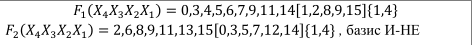
\includegraphics[]{task.png}
  \end{figure}
\end{center}

\section{Таблицы истинности}

\begin{center}
  \begin{tabular}{|c|c|c|c|c|c|c|}
    \hline
    № набора & \(X_4\) & \(X_3\) & \(X_2\) & \(X_1\) & \(F_1\) & \(F_2\) \\
    \hline
    0   & 0 & 0 & 0 & 0 & 1 & 0 \\
    \hline
    1   & 0 & 0 & 0 & 1 & * & * \\
    \hline
    2   & 0 & 0 & 1 & 0 & 0 & 1 \\
    \hline
    3   & 0 & 0 & 1 & 1 & 1 & 0 \\
    \hline
    4   & 0 & 1 & 0 & 0 & * & * \\
    \hline
    5   & 0 & 1 & 0 & 1 & 1 & 0 \\
    \hline
    6   & 0 & 1 & 1 & 0 & 1 & 1 \\
    \hline
    7   & 0 & 1 & 1 & 1 & 1 & 0 \\
    \hline
    8   & 1 & 0 & 0 & 0 & 0 & 1 \\
    \hline
    9   & 1 & 0 & 0 & 1 & 1 & 1 \\
    \hline
    10  & 1 & 0 & 1 & 0 & 0 & 0 \\
    \hline
    11  & 1 & 0 & 1 & 1 & 1 & 1 \\
    \hline
    12  & 1 & 1 & 0 & 0 & 0 & 0 \\
    \hline
    13  & 1 & 1 & 0 & 1 & 0 & 1 \\
    \hline
    14  & 1 & 1 & 1 & 0 & 1 & 0 \\
    \hline
    15  & 1 & 1 & 1 & 1 & 0 & 1 \\
    \hline
  \end{tabular}
\end{center}

Минимизируем данные функции используя карты Карно

Начнём с функии $F_1$
\begin{center}
  \begin{tabular}{|c|c|c|c|c|}
    \hline
    \(X_4 X_3 \backslash X_2 X_1\) & 00 & 01 & 11 & 10 \\
    \hline
    00 & 1  & *  & 1  & 0  \\
    \hline
    01 & *  & 1  & 1  & 1  \\
    \hline
    11 & 0  & 0  & 0  & 1  \\
    \hline
    10 & 0  & 1  & 1  & 0  \\
    \hline
  \end{tabular}
\end{center}

Тогда минимизированная функция имеет вид $$F_1 = \overline{X_4}\overline{X_2} + \overline{X_4}X_1 + \overline{X_3}X_1 + X_2X_3\overline{X_1}$$

Минимизируем функию $F_2$
\begin{center}
  \begin{tabular}{|c|c|c|c|c|}
    \hline
    \(X_4 X_3 \backslash X_2 X_1\) & 00 & 01 & 11 & 10 \\
    \hline
    00 & 0  & *  & 0  & 1  \\
    \hline
    01 & *  & 0  & 0  & 1  \\
    \hline
    11 & 0  & 1  & 1  & 1  \\
    \hline
    10 & 1  & 1  & 1  & 0  \\
    \hline
  \end{tabular}
\end{center}

Тогда минимизированная функция имеет вид $$F_2 = \overline{X_4}X_2\overline{X_1} + X_4\overline{X_3}\overline{X_2} + X_1X_4$$

\section{Построение логических схем}

По полученным уравнениям построим логические схемы.

Для функции 1

\begin{center}
  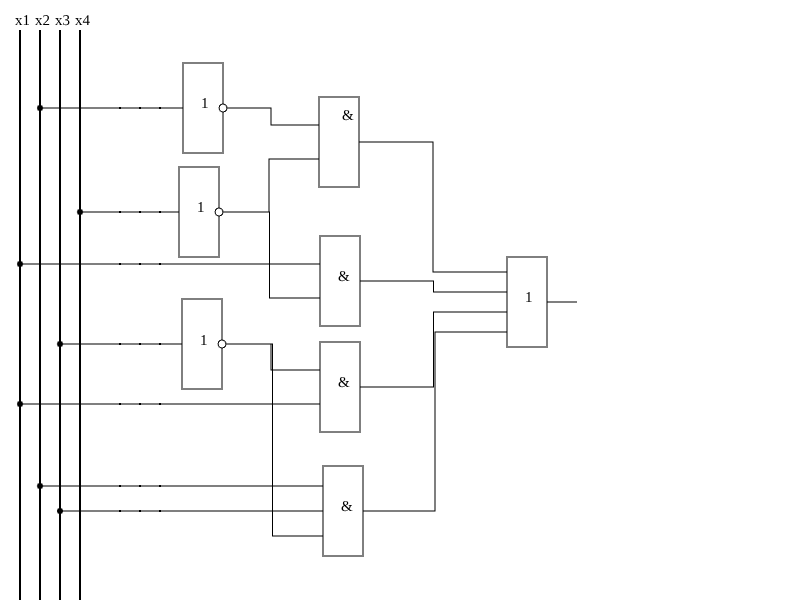
\includegraphics[width=0.8\textwidth]{logic1.png}
\end{center}

Для функции 2

\begin{center}
  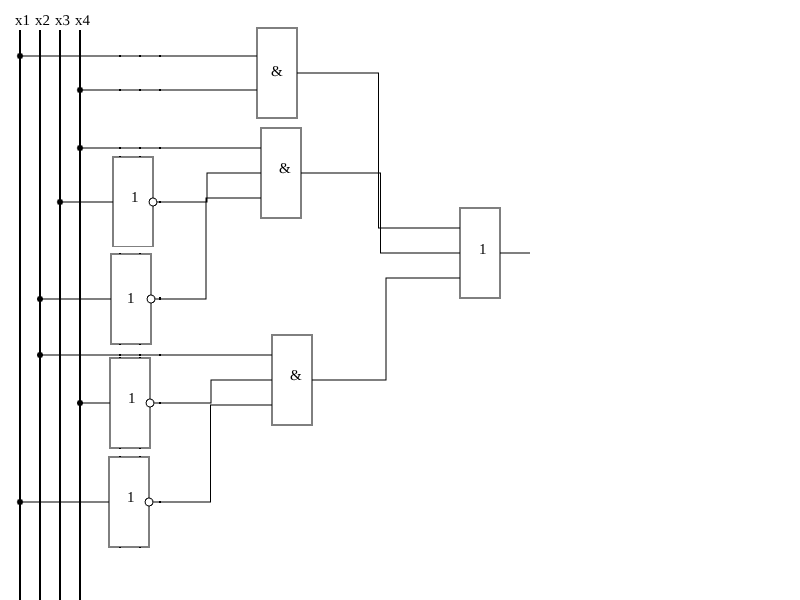
\includegraphics[width=0.8\textwidth]{logic2.png}
\end{center}

\section{Моделирование в multisim}

В результате моделирования были получены следующиие схемы.

\begin{center}
  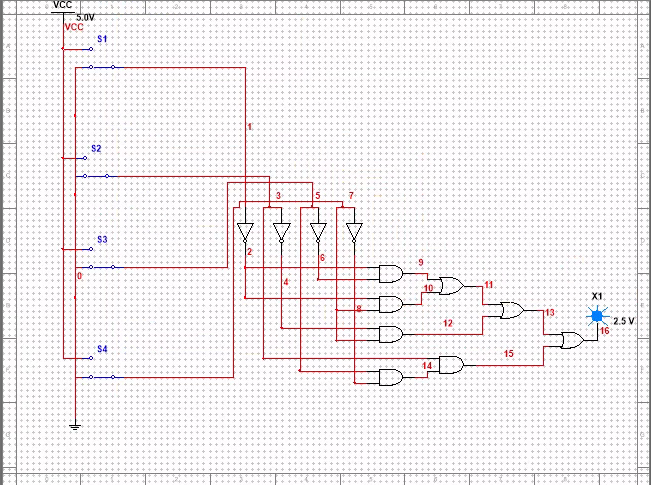
\includegraphics[width=0.8\textwidth]{scheme1.png}
\end{center}

\begin{center}
  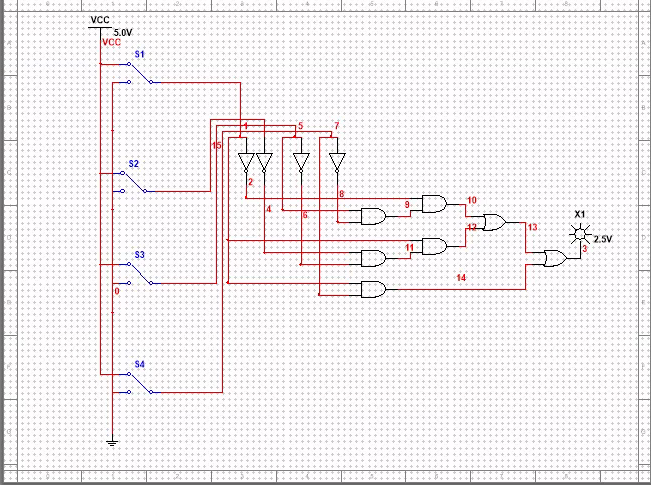
\includegraphics[width=0.8\textwidth]{scheme2.png}
\end{center}

В результате тестирования были получены следующие значения

\begin{center}
  \begin{tabular}{|c|c|c|c|c|c|c|}
    \hline
    № набора & \(X_4\) & \(X_3\) & \(X_2\) & \(X_1\) & \(F_1\) & \(F_2\) \\
    \hline
    0   & 0 & 0 & 0 & 0 & 1 & 0 \\
    \hline
    1   & 0 & 0 & 0 & 1 & 1 & 0 \\
    \hline
    2   & 0 & 0 & 1 & 0 & 0 & 1 \\
    \hline
    3   & 0 & 0 & 1 & 1 & 1 & 0 \\
    \hline
    4   & 0 & 1 & 0 & 0 & 1 & 0 \\
    \hline
    5   & 0 & 1 & 0 & 1 & 1 & 0 \\
    \hline
    6   & 0 & 1 & 1 & 0 & 1 & 1 \\
    \hline
    7   & 0 & 1 & 1 & 1 & 1 & 0 \\
    \hline
    8   & 1 & 0 & 0 & 0 & 0 & 1 \\
    \hline
    9   & 1 & 0 & 0 & 1 & 1 & 1 \\
    \hline
    10  & 1 & 0 & 1 & 0 & 0 & 0 \\
    \hline
    11  & 1 & 0 & 1 & 1 & 1 & 1 \\
    \hline
    12  & 1 & 1 & 0 & 0 & 0 & 0 \\
    \hline
    13  & 1 & 1 & 0 & 1 & 0 & 1 \\
    \hline
    14  & 1 & 1 & 1 & 0 & 1 & 0 \\
    \hline
    15  & 1 & 1 & 1 & 1 & 0 & 1 \\
    \hline
  \end{tabular}
\end{center}

Полученная эксперементальная таблица соответствует исходной, значит моделирование выполнено верно.

\section{Перевод полученных уравнений в базис И-НЕ и построение их логических схем}

Пользуясь законом Де-Моргана переведем уравнения в базис И-НЕ:

$$F_1 = \overline{\overline{\overline{X_4}\overline{X_2}} \cdot \overline{\overline{X_4}X_1} \cdot \overline{\overline{X_3}X_1} \cdot \overline{X_2X_3\overline{X_1}}}$$

\begin{center}
  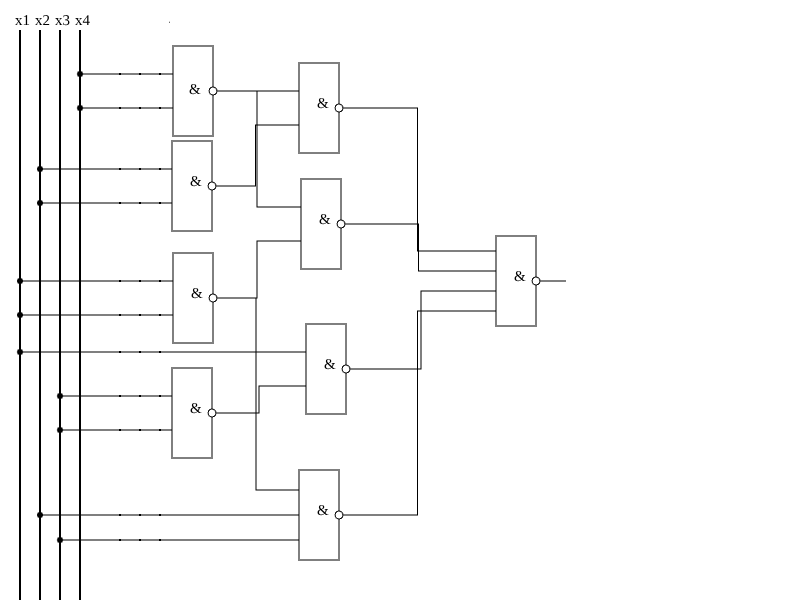
\includegraphics[width=0.8\textwidth]{logicnotand1.png}
\end{center}

$$F_2 = \overline{\overline{\overline{X_4}X_2\overline{X_1}} \cdot \overline{X_4\overline{X_3}\overline{X_2}} \cdot \overline{X_1X_4}}$$

\begin{center}
  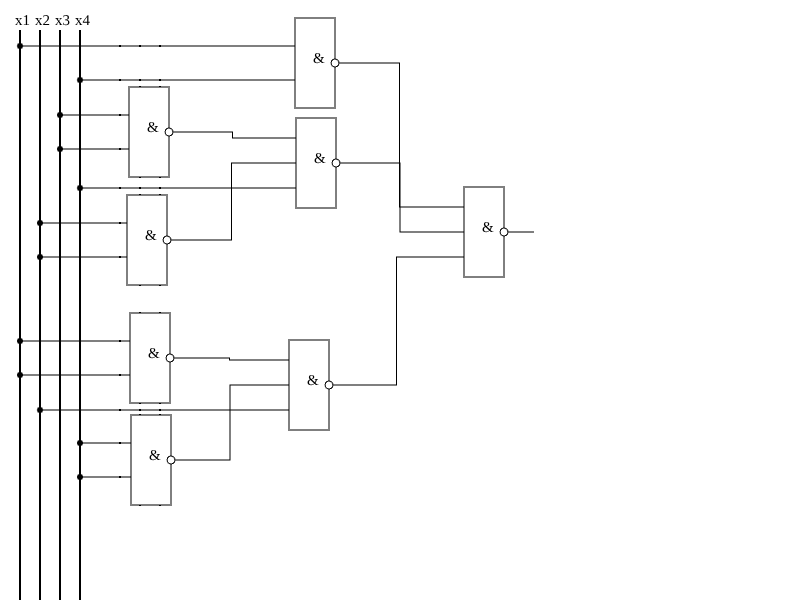
\includegraphics[width=0.8\textwidth]{logicnotand2.png}
\end{center}

\section{Тестирование построеных схем в базисе И-НЕ}

В среде моделирования NI Multisim были построены следующие схем:;

Для функции  $F_1$

\begin{center}
  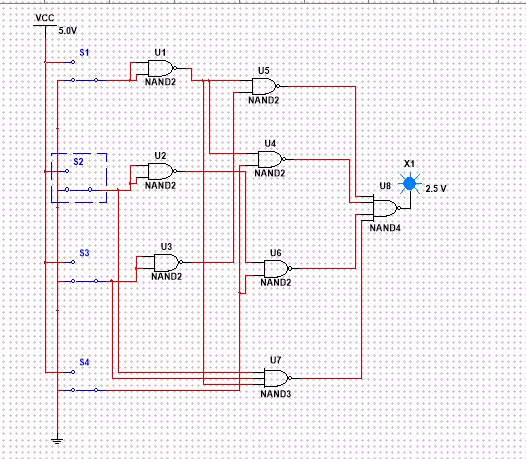
\includegraphics[width=0.8\textwidth]{schemenotand1.png}
\end{center}

Для функции  $F_2$

\begin{center}
  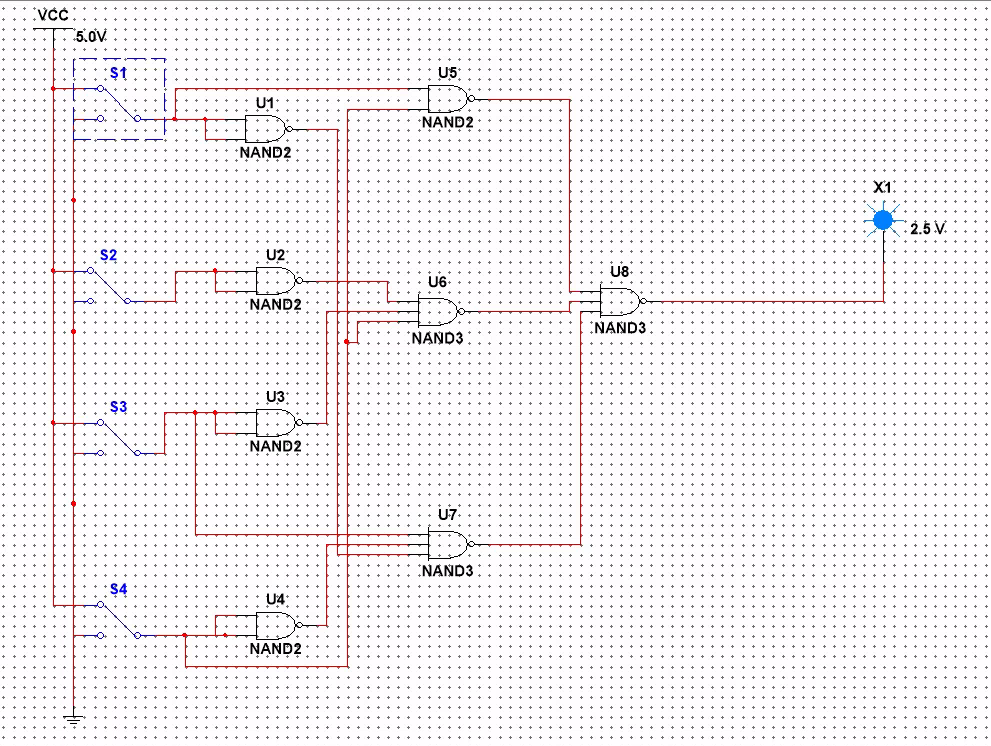
\includegraphics[width=0.8\textwidth]{schemenotand2.png}
\end{center}

В результате тестирования получена таблица истинности представленная ниже.

\begin{center}
  \begin{tabular}{|c|c|c|c|c|c|c|}
    \hline
    № набора & \(X_4\) & \(X_3\) & \(X_2\) & \(X_1\) & \(F_1\) & \(F_2\) \\
    \hline
    0   & 0 & 0 & 0 & 0 & 1 & 0 \\
    \hline
    1   & 0 & 0 & 0 & 1 & 1 & 0 \\
    \hline
    2   & 0 & 0 & 1 & 0 & 0 & 1 \\
    \hline
    3   & 0 & 0 & 1 & 1 & 1 & 0 \\
    \hline
    4   & 0 & 1 & 0 & 0 & 1 & 0 \\
    \hline
    5   & 0 & 1 & 0 & 1 & 1 & 0 \\
    \hline
    6   & 0 & 1 & 1 & 0 & 1 & 1 \\
    \hline
    7   & 0 & 1 & 1 & 1 & 1 & 0 \\
    \hline
    8   & 1 & 0 & 0 & 0 & 0 & 1 \\
    \hline
    9   & 1 & 0 & 0 & 1 & 1 & 1 \\
    \hline
    10  & 1 & 0 & 1 & 0 & 0 & 0 \\
    \hline
    11  & 1 & 0 & 1 & 1 & 1 & 1 \\
    \hline
    12  & 1 & 1 & 0 & 0 & 0 & 0 \\
    \hline
    13  & 1 & 1 & 0 & 1 & 0 & 1 \\
    \hline
    14  & 1 & 1 & 1 & 0 & 1 & 0 \\
    \hline
    15  & 1 & 1 & 1 & 1 & 0 & 1 \\
    \hline
  \end{tabular}
\end{center}

Полученная ттаблица соответствует заданию, значит построение логической и моделирование схемы выполнены верно.

\section{Минимизация количества логических эллемментов ДКЦУ}

В логических схемах для функций $F_1$ и $F_2$ используются общие логические эллементы, реализующие инверсию входных сигналов $X_n$. Объединим схемы для уменьшения количества логических эллементов, в результате получим следующую схему

\begin{center}
  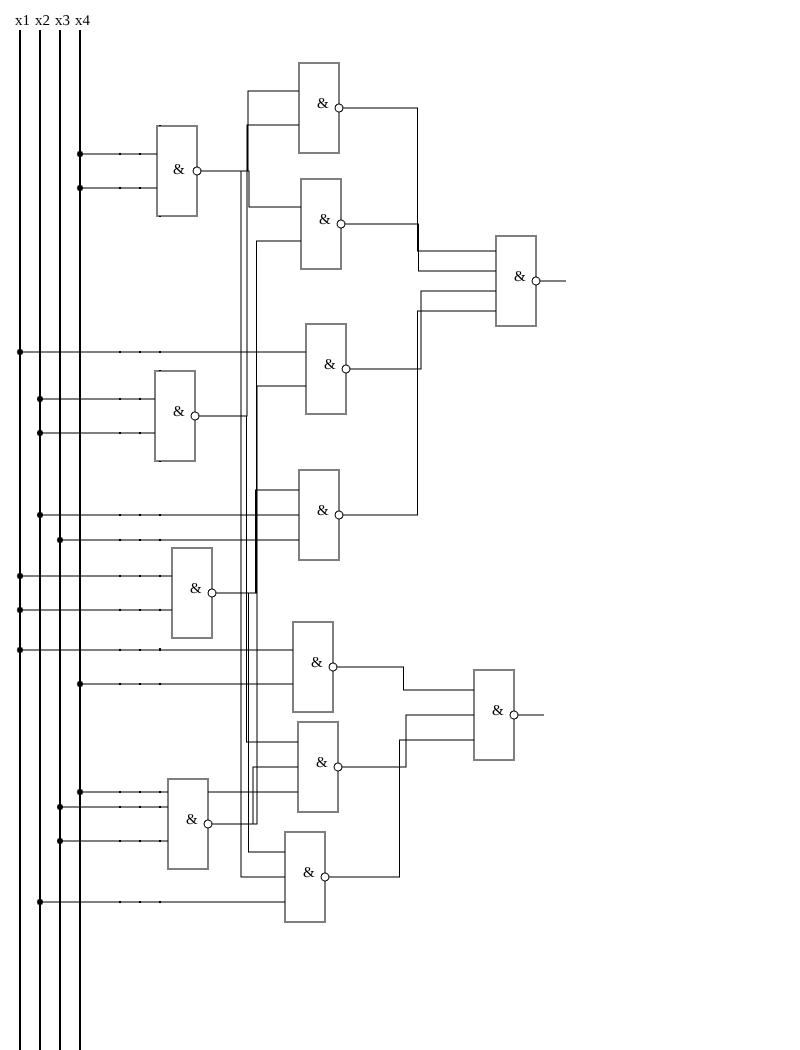
\includegraphics[width=0.8\textwidth]{logicnotandunit.png}
\end{center}

При моделирование этой схемы получаем следующую модель ДКЦУ

\begin{center}
  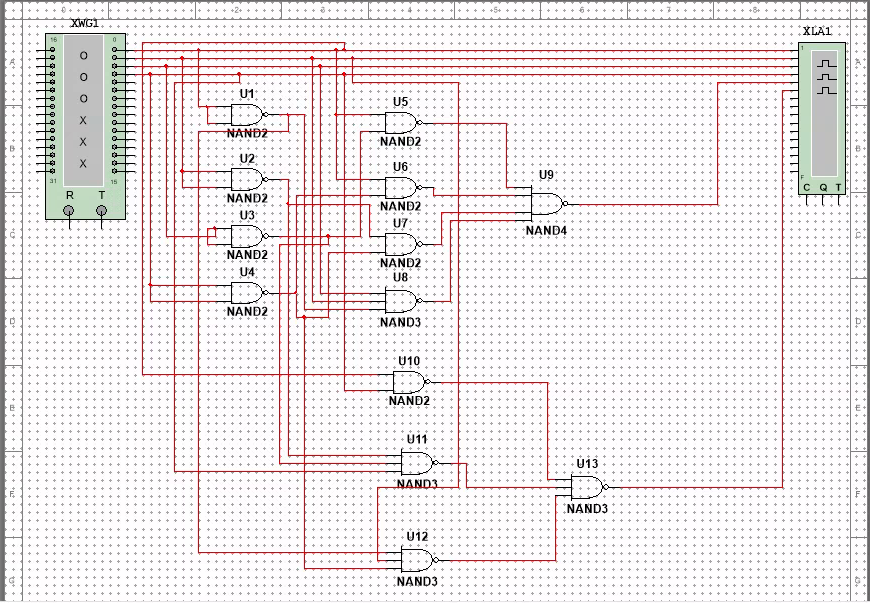
\includegraphics[width=0.8\textwidth]{schemetest.png}
\end{center}

Проверим полученную схему построив временную диаграмму

\begin{center}
  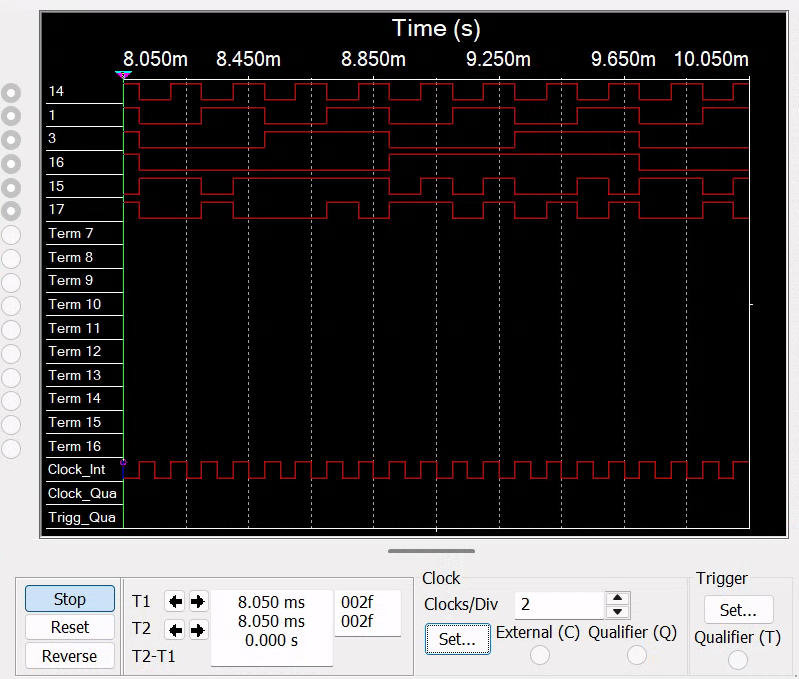
\includegraphics[width=0.8\textwidth]{timediagram.png}
\end{center}

И сравним ее с требуемой:

\begin{figure}[H]
  \centering

  \begin{tikztimingtable}[
      timing/slope=0,
      timing/dslope=0,
      xscale=1.2,
      yscale=1.2
    ]
    $X_4$ & 8L 8H \\
    $X_3$ & 4L 4H 4L 4H \\
    $X_2$ & 2L 2H 2L 2H 2L 2H 2L 2H \\
    $X_1$ & 1L 1H 1L 1H 1L 1H 1L 1H 1L 1H 1L 1H 1L 1H 1L 1H \\
    $F_1$ & 2H 1L 5H 1L 1H 1L 1H 2L 1H 1L \\
    $F_2$ & 2L 1H 3L 1H 1L 2H 1L 1H 1L 1H L H \\
    \extracode
    \begin{pgfonlayer}{background}

      % вертикальная сетка
      \foreach \x in {1,...,16}
      \draw[gray!40] (\x,0) -- (\x,-10);

      % горизонтальная сетка
      \foreach \y in {0,-1,-2,-3,-4,-5,-6, -7, -10}
      \draw[gray!40] (0,\y) -- (16,\y);

    \end{pgfonlayer}

  \end{tikztimingtable}

\end{figure}

\section{Выполнение жлектрической принципиальной схемы ДКЦУ}

Для выполнения электрической принципиальной схемы ДКЦУ будем использовать
микросхемы ТТЛ серии К155ЛАЗ 4 2 В И-НЕ. Основные электрические
параметры микросхем ТТЛ, следующие:

\begin{itemize}
  \item Высокий уровень сигнала (Н) находится в диапазоне 2,4 -5В, нижний – не более
    0,4 В.
  \item Входной ток низкого уровня составляет -1,6мА, высокого -0.04мА.
    Коэффициент разветвления по выходу равен 10.
  \item  Напряжение питания составляет 5,0 В ±10% В.
  \item Микросхемы серии 155: ЛА1, ЛА2, ЛА3, ЛА4, ЛЛ1, ЛЕ1, ЛЕ4, ЛН2, ЛР4,1, ЛР4
    изготавливают в 14- выводном корпусе рис.2.14. Выводы нумеруют
    относительно ключа (выемки в корпусе), на виде сверху – против часовой
    стрелки
\end{itemize}

\begin{center}
  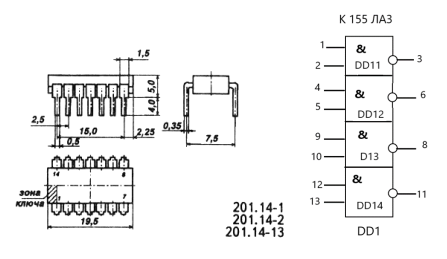
\includegraphics{K155.png}
\end{center}

Эта микросхема содержит четыре логических элемента И-НЕ, изготовленные в
одном корпусе. На рисунке микросхемы не указаны вывод7 («земля») и вывод
14(+5В), через которые подводится питание микросхеме.
Для синтезируемого КЦУ необходимо 5 микросхем К155ЛА3 (21 ЛЭ И-НЕ) и один
соединитель РМ-В. Он устанавливается на плате. Его внутренние выводы (13 штук)
располагаются в отверстиях платы в отверстиях платы под корпус соединителя. На
рисунке ниже представлена электрическая принципиальная схема спроектированного
комбинационного цифрового устройства.

\begin{center}
  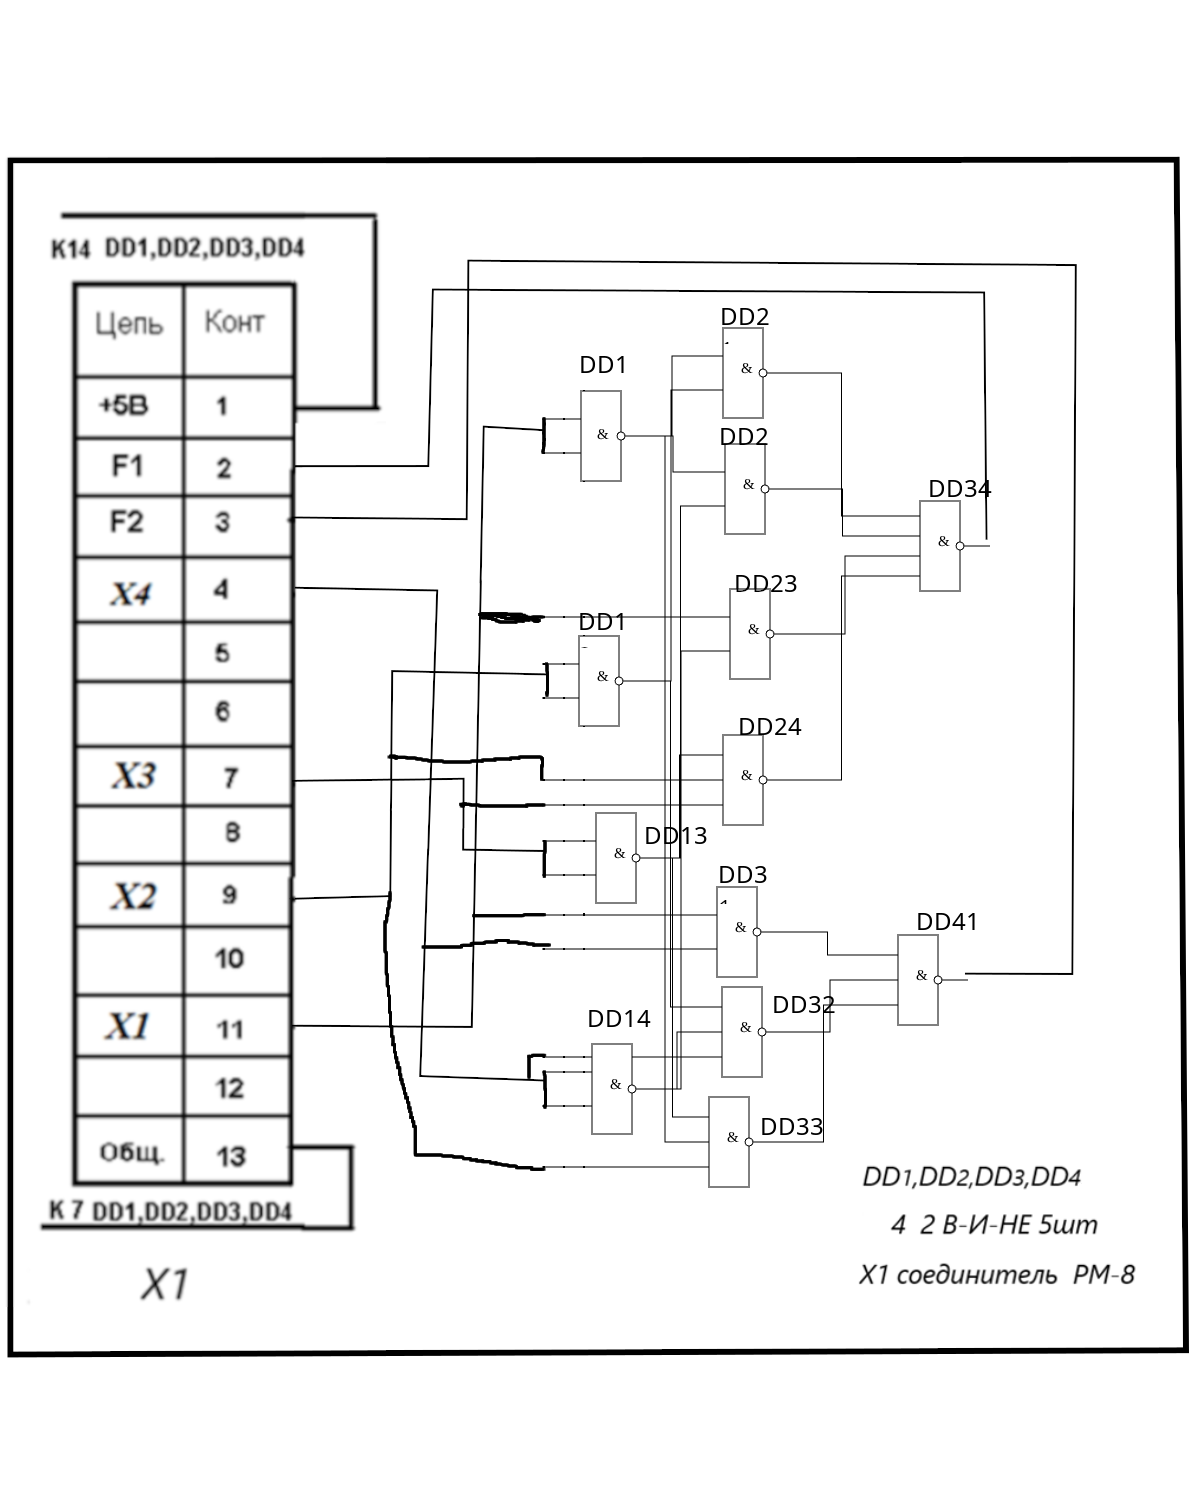
\includegraphics[width=0.8\textwidth]{DKCU.png}
\end{center}

\section{Расчет быстродействия ДКЦУ  }

Время задержки КЦУ оцениваем суммой задержек на отдельных логических
элементах по пути с наибольшим их числом. В нашем случае сигнал проходит шесть
логических элементов:

$$ t_\text{зад} = t_\text{зад1} \cdot 3 = 30 \text{нс} \cdot 3 = 90 \text{нс} $$
\end{document}